\documentclass[12pt,a4paper,UTF8]{article}
\usepackage{amsmath,amssymb}
\usepackage{enumitem}
\usepackage{graphicx}
\usepackage{geometry}
\usepackage{ctex}
\usepackage{booktabs}
\usepackage{tikz}
\usepackage{tocloft}    % 目录美化
\usepackage{hyperref}   % 目录超链接（核心包）
\usetikzlibrary{calc,arrows}
\geometry{margin=2.5cm}

% 超链接样式（不显示彩色边框，更美观）
\hypersetup{
    colorlinks=true,
    linkcolor=black,
    citecolor=black,
    urlcolor=blue
}

% 逻辑符号
\newcommand{\xorop}{\oplus}
\newcommand{\notop}{\prime}
\newcommand{\andop}{\cdot}
\newcommand{\orop}{+}

\begin{document}

% 引入封面
\begin{titlepage}
    \centering
    % 顶部间距调整，布局更均衡
    \vspace*{3cm}
    
    % 主标题
    {\Huge \bfseries 数字电路与逻辑设计 \par}
    \vspace{1.5cm}
    
    % 副标题
    {\Large \bfseries 作业合集 \par}
    \vspace{2cm}
    % 作者信息
    {\Large 作者：浮萍 \par}
    \vspace{0.5cm}
    
    % 版本号
    {\large 版本：1.0 完整版 \par}
    \vspace{0.5cm}
    
    % 联系方式
    {\large 邮箱：3071974740@qq.com \par}
    \vspace{0.5cm}
    
    % GitHub链接
    {\large GitHub：https://github.com/Duckweed-yhb \par}
    
    \vspace{3cm}
    % 生成日期
    {\large \today \par}
\end{titlepage}

% 目录（带超链接）
\newpage
\tableofcontents
\newpage

% 各章节内容
\section{第一章 数制和码制 作业}

\subsection*{补充题}
将 $(01111001)_2$ 8421BCD码转换为等值的二进制数：
\[
(01111001)_{8421\text{BCD}} = (\underline{1001110001})_2
\]
\textbf{解答：}
8421BCD码 $(0111\ 1001)_\text{BCD} = 79_{10}$，
将 $79$ 转为二进制：$79 = 64+8+4+2+1 = (1001110001)_2$。

\subsection{题1.1}
为了将600份文件顺序编码，如果采用二进制代码，最少需要用几位？如果改用八进制或十六进制代码，则最少各需要用几位？

\textbf{解答：}
需要满足 $2^n \ge 600$。
\begin{itemize}
    \item 二进制：$2^9=512<600$，$2^{10}=1024\ge600$，故最少 \textbf{10 位}。
    \item 八进制：$8^4=4096\ge600$，故最少 \textbf{4 位}。
    \item 十六进制：$16^3=4096\ge600$，故最少 \textbf{3 位}。
\end{itemize}

\subsection{题1.4 (4)}
将下列二进制数转换为等值的十进制数：
\begin{enumerate}
    \item $(1001.0101)_2$
\end{enumerate}
\textbf{解答：}
\[
\begin{aligned}
(1001.0101)_2 &= 1\times2^3 + 0\times2^2 + 0\times2^1 + 1\times2^0 + 0\times2^{-1} + 1\times2^{-2} + 0\times2^{-3} + 1\times2^{-4} \\
&= 8 + 0 + 0 + 1 + 0 + 0.25 + 0 + 0.0625 \\
&= \mathbf{9.3125}_{10}
\end{aligned}
\]

\subsection{题1.5 (4)}
将下列二进制数转换为等值的八进制数和十六进制数：
\begin{enumerate}
    \item $(101100.110011)_2$
\end{enumerate}
\textbf{解答：}
\begin{align*}
(101100.110011)_2 &= (010\ 110\ 0.110\ 011)_2 = \mathbf{(54.63)_8} \\
(101100.110011)_2 &= (0010\ 1100.1100\ 1100)_2 = \mathbf{(2C.CC)_{16}}
\end{align*}

\subsection{题1.9 (1)、(2)}
将下列十进制数转换为等值的二进制数和十六进制数。要求二进制数保留小数点以后4位有效数字：
\begin{enumerate}
    \item $(25.7)_{10}$
    \textbf{解答：}
    整数部分：$25 = (11001)_2$
    小数部分：$0.7 \approx (0.1011)_2$
    故：
    \[
    (25.7)_{10} = \mathbf{(11001.1011)_2} = \mathbf{(19.B)_{16}}
    \]

    \item $(188.875)_{10}$
    \textbf{解答：}
    整数部分：$188 = (10111100)_2$
    小数部分：$0.875 = (0.111)_2$
    故：
    \[
    (188.875)_{10} = \mathbf{(10111100.1110)_2} = \mathbf{(BC.E)_{16}}
    \]
\end{enumerate}

\subsection{题1.12 (1)、(3)}
用8位的二进制补码表示下列十进制数：
\begin{enumerate}
    \item $+17$
    \textbf{解答：}
    正数补码等于原码：
    \[
    +17 \Rightarrow \mathbf{(00010001)_2}
    \]

    \item $-13$
    \textbf{解答：}
    原码：$10001101$，反码：$11110010$，补码：$11110011$
    \[
    -13 \Rightarrow \mathbf{(11110011)_2}
    \]
\end{enumerate}
\newpage

\section{第二章 逻辑代数基础 作业}

\subsection{题2.2 证明下列逻辑恒等式}
\begin{enumerate}
    \item $AB' + B + A'B = A + B$

    \textbf{证明：}
    \begin{align*}
    \text{左边} &= AB' + B + A'B \\
              &= AB' + B(1 + A') \\
              &= AB' + B \\
              &= A + B = \text{右边}
    \end{align*}

    \item $(A + C')(B + D)(B + D') = AB + BC'$

    \textbf{证明：}
    \begin{align*}
    \text{左边} &= (A + C') \cdot \big[(B + D)(B + D')\big] \\
              &= (A + C') \cdot B \\
              &= AB + BC' = \text{右边}
    \end{align*}

    \item $A'B'C' + A(B + C) + BC = (AB'C' + A'B'C + A'BC')'$

    \textbf{证明：}
    \begin{align*}
    \text{右边} &= (AB'C')'(A'B'C)'(A'BC')' \\
                &= (A' + B + C)(A + B + C')(A + B' + C) \\
                &= A'B'C' + AB + AC + BC \\
                &= A'B'C' + A(B + C) + BC = \text{左边}
    \end{align*}
\end{enumerate}

\subsection{题2.6 写出图P2.6(a)(b)的输出逻辑函数式}
\begin{figure}[ht]
    \centering
    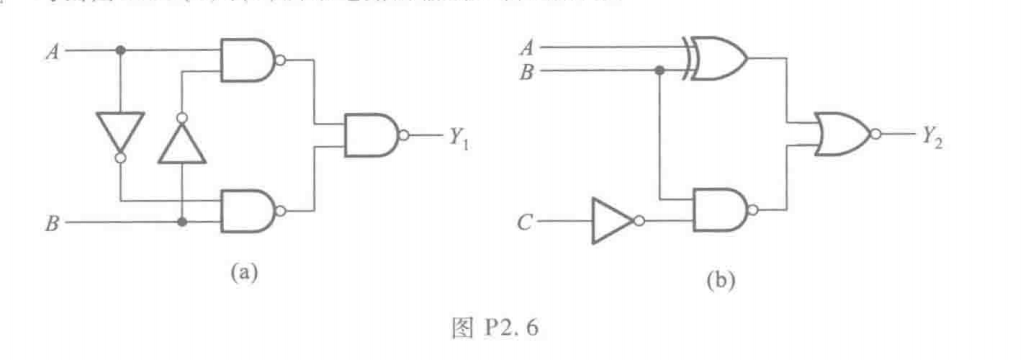
\includegraphics[width=0.8\textwidth]{2.6.png}
    \caption{图P2.6 逻辑电路图}
\end{figure}

\textbf{解：}
\begin{align*}
Y_a &= \overline{\overline{A\cdot B'} \cdot \overline{A'\cdot B}} = A \oplus B \\
Y_b &= \overline{(A\oplus B) + \overline{B C'}} = AB\overline{C}
\end{align*}

\subsection{题2.8 根据波形图写出真值表与逻辑函数式}
\begin{figure}[ht]
    \centering
    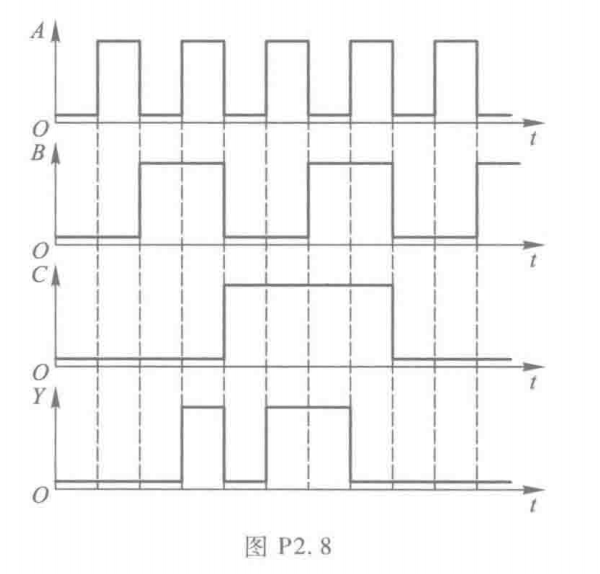
\includegraphics[width=0.8\textwidth]{2.8.png}
    \caption{图P2.8 波形图}
\end{figure}

\textbf{解：}
由波形图可得
\[
Y = \sum m(3,6) = A'BC + ABC'
\]

\subsection{题2.10 化为最小项之和形式}
\begin{enumerate}
    \item $Y = A'BC + AC + B'C$

    \textbf{解：}
    \begin{align*}
    Y &= A'BC + AC(B+B') + B'C(A+A') \\
      &= A'BC + ABC + AB'C + A'B'C \\
      &= \sum m(1,3,6,7)
    \end{align*}

    \item $Y = AB'C'D + BCD + A'D$

    \textbf{解：}
    \begin{align*}
    Y &= AB'C'D + BCD(A+A') + A'D(B+B')(C+C') \\
      &= \sum m(1,3,5,7,9,15)
    \end{align*}

    \item $Y = A + B + CD$

    \textbf{解：}
    \[
    Y = \sum m(3,4,5,6,7,8,9,10,11,12,13,14,15)
    \]

    \item $Y = AB + ((BC)'(C' + D'))'$

    \textbf{解：}
    \begin{align*}
    Y &= AB + BC + CD \\
      &= \sum m(3,6,7,11,12,13,14,15)
    \end{align*}
\end{enumerate}

\subsection{题2.12 化简逻辑函数}
\begin{enumerate}
    \item $ACD' + D'$

    \textbf{解：}
    \[
    Y = D'(AC + 1) = D'
    \]

    \item $AB' + AC + BC$

    \textbf{解：}
    \[
    Y = AB' + BC
    \]

    \item $E'F' + E'F + EF' + EF$

    \textbf{解：}
    \[
    Y = E'(F'+F) + E(F'+F) = E' + E = 1
    \]

    \item $A'BC + (A + B')C$

    \textbf{解：}
    \[
    Y = A'BC + AC + B'C = C(A'B + A + B') = C
    \]
\end{enumerate}

\subsection{题2.13 化为最简与或式}
\begin{enumerate}
    \item $Y = AB'C + A' + B + C'$

    \textbf{解：}
    \[
    Y = A' + B + C' + AB'C = A' + B + C' + C = 1
    \]

    \item $Y = AB'CD + ABD + AC'D$

    \textbf{解：}
    \[
    Y = AD(B'C + B + C') = AD
    \]

    \item $Y = AC(C'D + A'B) + BC((B' + AD)' + CE)'$

    \textbf{解：}
    \begin{align*}
    Y &= AC'D + ABCD(C' + E') \\
      &= AC'D
    \end{align*}

    \item $Y = A + (B + C')'(A + B' + C)(A + B + C)$

    \textbf{解：}
    \begin{align*}
    Y &= A + B'C(A + C) \\
      &= A + B'C
    \end{align*}

    \item $Y = AC + AC'D + AB'E'F + B(D \oplus E) + BC'DE' + BC'D'E + ABE'F$

    \textbf{解：}
    \begin{align*}
    Y &= A(C + C'D) + AE'F + B(D \oplus E)(1 + C') \\
      &= AC + AD + AE'F + B(D \oplus E)
    \end{align*}
\end{enumerate}

\subsection{题2.15 卡诺图化简}
\begin{enumerate}
    \item $Y_1 = C + ABC$

    \textbf{解：}
    \[
    Y_1 = C(1 + AB) = C
    \]

    \item $Y_2 = AB'C + BC + A'BC'D$

    \textbf{解：}
    \[
    Y_2 = C
    \]

    \item $Y_3(A,B,C) = \sum m(1,2,3,7)$

    \textbf{解：}
    \[
    Y_3 = A'C + BC
    \]

    \item $Y_4(A,B,C,D) = \sum m(0,1,2,3,4,6,8,9,10,11,14)$

    \textbf{解：}
    \[
    Y_4 = B' + CD'
    \]
\end{enumerate}

\subsection{题2.16 卡诺图化简}
\begin{enumerate}
    \item $Y = AB' + A'C + BC + C'D$

    \textbf{解：}
    \[
    Y = A'C + AB' + C'D
    \]

    \item $Y = A'B' + BC' + A' + B' + ABC$

    \textbf{解：}
    \begin{align*}
    Y &= A'(1 + B') + B'(1 + A) + BC' + ABC \\
      &= A' + B' + C
    \end{align*}
\end{enumerate}

\subsection{题2.18 写出逻辑式并化简}
\begin{figure}[ht]
    \centering
    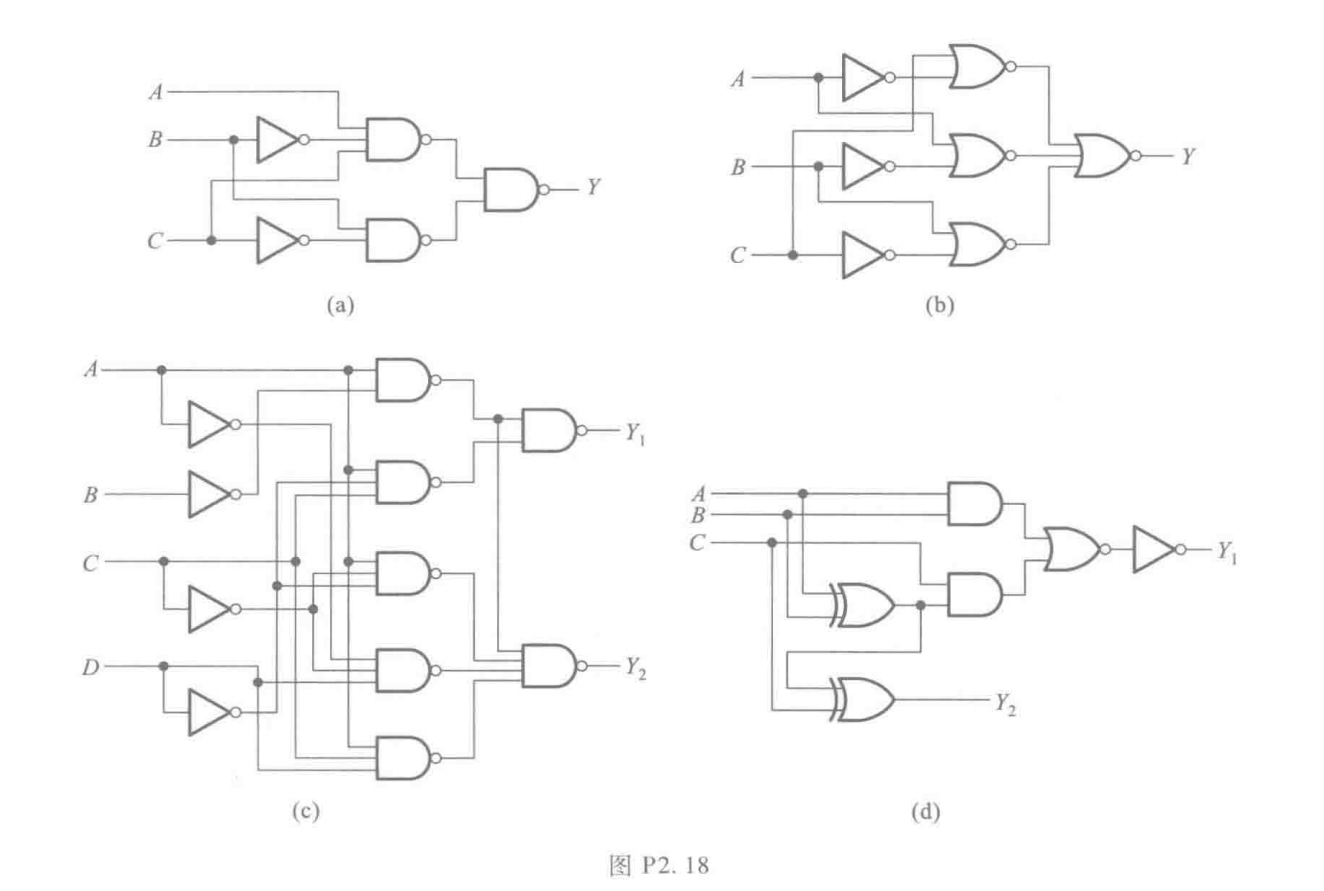
\includegraphics[width=0.85\textwidth]{2.18.png}
    \caption{图P2.18 逻辑图}
\end{figure}

\textbf{解：}
\begin{align*}
Y_a &= A\overline{B} + \overline{C} \\
Y_b &= \overline{B} + AC \\
Y_c &= AC + \overline{B}D
\end{align*}

\subsection{题2.20 (1) 带约束项化简}
\[
Y_1 = AB'C' + ABC + A'B'C + A'BC',\quad A'B'C' + A'BC = 0
\]

\textbf{解：}
利用约束项合并卡诺图：
\[
Y_1 = AC + B'C'
\]

\subsection{题2.21 (1)(3) 带无关项化简}
\begin{enumerate}
    \item $Y_1 = \sum m(0,1,2,4) + d(5,6)$

    \textbf{解：}
    \[
    Y_1 = A' + B'C'
    \]

    \item $Y_3 = \sum m(3,5,6,7,10) + d(0,1,2,4,8)$

    \textbf{解：}
    \[
    Y_3 = A'B + AC + A'D
    \]
\end{enumerate}

\subsection{题2.24 多输出函数化简}
\begin{align*}
Y_1 &= \sum m(0,1,8,9,10,12,13,14) \\
Y_2 &= \sum m(0,1,2,3,6,7,10,14)
\end{align*}

\textbf{解：}
\[
Y_1 = B'C' + AC' + ABD',\quad
Y_2 = A'B' + A'C + BC'D'
\]

\subsection{题2.26 化为与非–与非式}
\begin{enumerate}
    \item $Y = AB + BC + AC$

    \textbf{解：}
    \[
    Y = \overline{\overline{AB} \cdot \overline{BC} \cdot \overline{AC}}
    \]

    \item $Y = (A' + B)(A + B')C + (BC)'$

    \textbf{解：}
    \begin{align*}
    Y &= AB'C + A'BC + B' + C' \\
      &= B' + C' = \overline{\overline{B'} \cdot \overline{C'}}
    \end{align*}

    \item $Y = (ABC' + AB'C + A'BC)'$

    \textbf{解：}
    \[
    Y = \overline{\overline{ABC'} \cdot \overline{AB'C} \cdot \overline{A'BC}}
    \]

    \item $Y = A(BC)' + ((AB')' + A'B' + BC)'$

    \textbf{解：}
    \begin{align*}
    Y &= AB' + AC' \\
      &= \overline{\overline{AB'} \cdot \overline{AC'}}
    \end{align*}
\end{enumerate}
\newpage

% 门电路习题 —— 完整解答子文件
% 可直接在主文件中 \input{problems_sub.tex} 引入
% 需主文档提前加载：\usepackage{tikz}

\section{第三章 门电路 作业}

\subsection{题3.3：复合门作反相器的可行性}
\subsubsection{题目}
试说明能否将与非门、或非门、异或门当做反相器使用？如果可以，各输入端应如何连接？

\subsubsection{解答}
\begin{enumerate}
    \item \textbf{与非门作反相器}：可以。
    \begin{itemize}
        \item 逻辑表达式：$Y = \overline{A \cdot B}$，要实现$Y = \overline{A}$，只需令$B = 1$（接高电平），此时$Y = \overline{A \cdot 1} = \overline{A}$。
        \item 连接方式：一个输入端接信号，其余输入端全部接高电平。
    \end{itemize}
    
    \item \textbf{或非门作反相器}：可以。
    \begin{itemize}
        \item 逻辑表达式：$Y = \overline{A + B}$，要实现$Y = \overline{A}$，只需令$B = 0$（接低电平），此时$Y = \overline{A + 0} = \overline{A}$。
        \item 连接方式：一个输入端接信号，其余输入端全部接低电平。
    \end{itemize}
    
    \item \textbf{异或门作反相器}：可以。
    \begin{itemize}
        \item 逻辑表达式：$Y = A \oplus B = A\overline{B} + \overline{A}B$，要实现$Y = \overline{A}$，只需令$B = 1$（接高电平），此时$Y = A \oplus 1 = \overline{A}$。
        \item 连接方式：一个输入端接信号，另一个输入端接高电平。
    \end{itemize}
\end{enumerate}

\subsection{题3.7(b)：CMOS门电路分析}
\subsubsection{题目}
试分析下图中电路的逻辑功能，写出输出的逻辑函数式。

\begin{center}
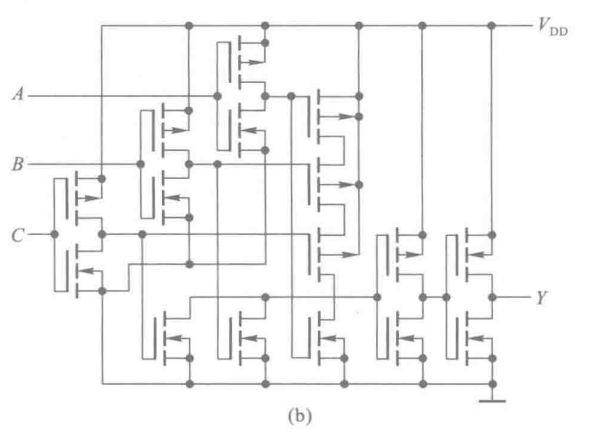
\includegraphics[width=0.6\textwidth]{3.7.b.png}
\end{center}
\textbf{题3.7(b)电路图}

\subsubsection{解答}
该电路为CMOS与或非门结构，PMOS管并联、NMOS管串联的结构实现与或非逻辑。
\begin{itemize}
    \item 逻辑表达式：
\[
Y = \overline{AB + C}
\]
\item 当$AB=1$或$C=1$时，对应NMOS管导通，PMOS管截止，输出低电平；
\item 当$AB=0$且$C=0$时，PMOS管导通，NMOS管截止，输出高电平。
\end{itemize}

\subsection{题3.7(d)：CMOS门电路分析}
\subsubsection{题目}
试分析下图中电路的逻辑功能，写出输出的逻辑函数式。

\begin{center}
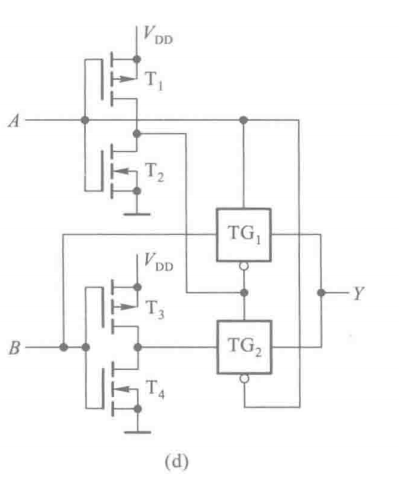
\includegraphics[width=0.5\textwidth]{3.7.d.png}
\end{center}
\textbf{题3.7(d)电路图}

\subsubsection{解答}
该电路由CMOS反相器和传输门组成，是一个二选一数据选择器结构：
\begin{itemize}
    \item 当$B=0$时，传输门$TG_1$导通，$TG_2$截止，$Y = A$；
    \item 当$B=1$时，传输门$TG_2$导通，$TG_1$截止，$Y = \overline{A}$；
    \item 逻辑表达式：
\[
Y = \overline{B}A + B\overline{A} = A \oplus B
\]
\end{itemize}

\subsection{题3.8：输出电压波形分析}
\subsubsection{题目}
试画出下图(a)、(b)两个电路的输出电压波形，输入电压波形如图(c)所示。

\begin{center}
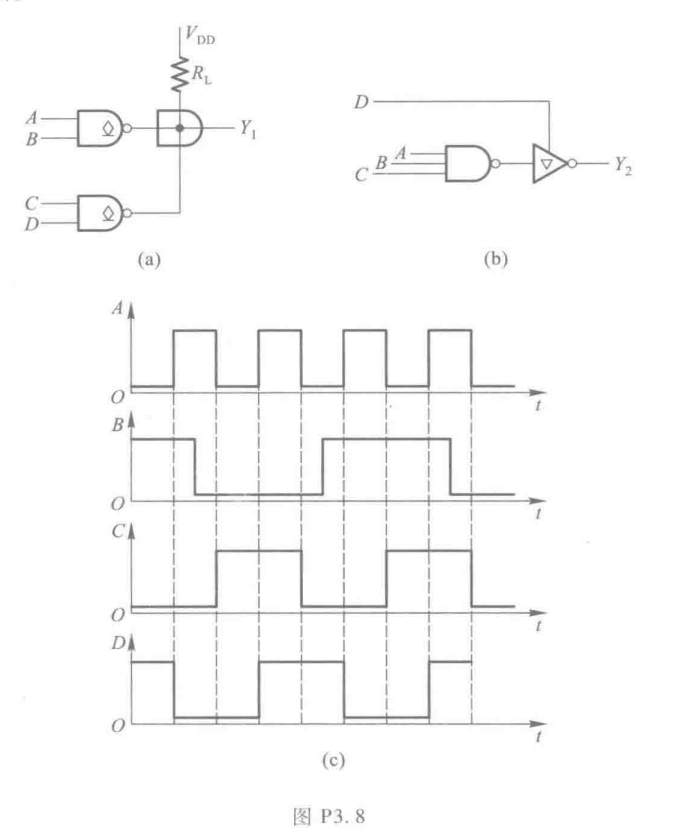
\includegraphics[width=0.7\textwidth]{3.8.png}
\end{center}
\textbf{题3.8电路图与输入波形}

\subsubsection{解答}
\begin{enumerate}
    \item \textbf{电路(a)：OC与非门线与结构}
    \begin{itemize}
        \item 逻辑表达式：$Y_1 = \overline{AB} \cdot \overline{CD} = \overline{AB + CD}$
        \item 输出波形：当$AB=1$或$CD=1$时，输出低电平；否则输出高电平。
    \end{itemize}

    \item \textbf{电路(b)：与非门+三态反相器}
    \begin{itemize}
        \item 逻辑表达式：当使能端$D=1$时，三态门使能，$Y_2 = \overline{ABC}$；当$D=0$时，三态门高阻。
        \item 输出波形：$D=1$时，$Y_2 = \overline{ABC}$；$D=0$时，输出高阻。
    \end{itemize}
\end{enumerate}

% 插入TikZ波形图
\begin{center}
\begin{tikzpicture}[>=stealth,scale=0.85,line width=0.7pt]
    % 时间轴
    \draw[->] (0,0) -- (17,0) node[right] {$t$};
    \foreach \x in {1,3,...,15} \draw (\x,0) -- (\x,-0.3);

    % 信号 A
    \draw (0,2) -- (1,2) -- (1,3) -- (3,3) -- (3,2) -- (5,2) -- (5,3) -- (7,3) -- (7,2) -- (9,2) -- (9,3) -- (11,3) -- (11,2) -- (13,2) -- (13,3) -- (15,3) -- (15,2);
    \node[left] at (0,2.5) {$A$};

    % 信号 B
    \draw (0,4) -- (2,4) -- (2,5) -- (4,5) -- (4,4) -- (6,4) -- (6,5) -- (8,5) -- (8,4) -- (10,4) -- (10,5) -- (12,5) -- (12,4) -- (14,4) -- (14,5) -- (16,5) -- (16,4);
    \node[left] at (0,4.5) {$B$};

    % 信号 C
    \draw (0,6) -- (4,6) -- (4,7) -- (8,7) -- (8,6) -- (12,6) -- (12,7) -- (16,7) -- (16,6);
    \node[left] at (0,6.5) {$C$};

    % 信号 D
    \draw (0,8) -- (2,8) -- (2,9) -- (6,9) -- (6,8) -- (10,8) -- (10,9) -- (14,9) -- (14,8);
    \node[left] at (0,8.5) {$D$};

    % 输出 Y1 (线与)
    \draw[red, thick]
    (0,10) -- (2,10)
    -- (2,9)  -- (4,9)
    -- (4,10) -- (6,10)
    -- (6,9)  -- (8,9)
    -- (8,10) -- (10,10)
    -- (10,9) -- (12,9)
    -- (12,10) -- (16,10);
    \node[left, red] at (0,9.5) {$Y_1$};

    % 输出 Y2 (三态)
    \draw[blue, thick]
    (0,12) -- (2,12)
    -- (2,11.5) -- (6,11.5) node[midway, fill=white] {高阻}
    -- (6,12) -- (8,12)
    -- (8,11.5) -- (12,11.5) node[midway, fill=white] {高阻}
    -- (12,12) -- (14,12)
    -- (14,11.5) -- (16,11.5);
    \node[left, blue] at (0,11.5) {$Y_2$};
\end{tikzpicture}
\end{center}

\subsection{题3.12：CMOS门电路输出电平判断}
\subsubsection{题目}
说明图中各门电路的输出是高电平还是低电平。已知它们都是74HC系列的CMOS电路。

\begin{center}
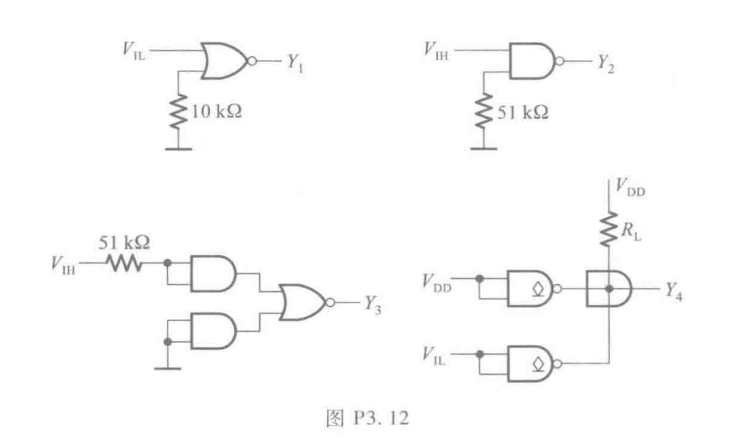
\includegraphics[width=0.6\textwidth]{3.12.png}
\end{center}
\textbf{题3.12电路图}

\subsubsection{解答}
CMOS电路输入阻抗极高，输入通过电阻接地时，电阻上无电流，输入端电位为0V；接高电平通过电阻时，输入端电位为高电平。
\begin{enumerate}
    \item $Y_1$：或非门，输入为$V_{IL}$和$0V$（通过10k$\Omega$电阻接地），$Y_1 = \overline{V_{IL} + 0} = \overline{0} = 1$（高电平）。
    \item $Y_2$：与非门，输入为$V_{IH}$和$0V$（通过51k$\Omega$电阻接地），$Y_2 = \overline{V_{IH} \cdot 0} = \overline{0} = 1$（高电平）。
    \item $Y_3$：两个与非门输入分别为$V_{IH}$和0、1，输出为$\overline{V_{IH} \cdot 0} = 1$和$\overline{1 \cdot 1} = 0$，再经或非门，$Y_3 = \overline{1 + 0} = 0$（低电平）。
    \item $Y_4$：两个OC门线与，输入分别为$V_{DD}$和$V_{IL}$，输出为$\overline{V_{DD} \cdot V_{DD}} = 0$和$\overline{V_{IL} \cdot V_{IL}} = 1$，线与后$Y_4 = 0 \cdot 1 = 0$（低电平）。
\end{enumerate}

\subsection{题3.13：TTL与非门输入电压测量}
\subsubsection{题目}
试说明在下列情况下，用万用表测量下图中的$v_{I2}$端得到的电压各为多少：
\begin{enumerate}
    \item $v_{I1}$悬空；
    \item $v_{I1}$接低电平(0.2V)；
    \item $v_{I1}$接高电平(3.2V)；
    \item $v_{I1}$经51$\Omega$电阻接地；
    \item $v_{I1}$经10k$\Omega$电阻接地。
\end{enumerate}
图中的与非门为74系列的TTL电路，万用表使用5V量程，内阻为20k$\Omega$/V。

\begin{center}
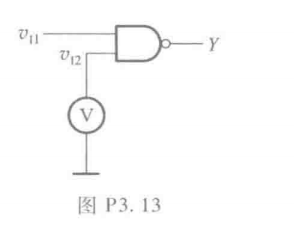
\includegraphics[width=0.3\textwidth]{3.13.png}
\end{center}
\textbf{题3.13电路图}

\subsubsection{解答}
TTL与非门输入级为多发射极三极管，输入特性存在开门/关门电平：
\begin{enumerate}
    \item $v_{I1}$悬空：相当于输入高电平，三极管导通，$v_{I2} \approx 1.4V$（PN结压降之和）。
    \item $v_{I1}=0.2V$：三极管基极电位被钳位，$v_{I2} = 0.2V + 0.7V = 0.9V$。
    \item $v_{I1}=3.2V$：三极管导通，$v_{I2} \approx 1.4V$。
    \item $v_{I1}$经51$\Omega$接地：输入电流在电阻上压降小，$v_{I1}$等效低电平，$v_{I2} \approx 0.9V$。
    \item $v_{I1}$经10k$\Omega$接地：电阻大于开门电阻，$v_{I1}$等效高电平，$v_{I2} \approx 1.4V$。
\end{enumerate}

\subsection{题3.17：TTL或非门扇出数计算}
\subsubsection{题目}
在下图所示由74系列或非门组成的电路中，试求门$G_M$能驱动多少同样的或非门。要求$G_M$输出的高、低电平满足$V_{OH} \ge 3.2V, V_{OL} \le 0.4V$。或非门每个输入端的输入电流为$I_{IL} \le -1.6mA, I_{IH} \le 40\mu A$。$V_{OL} \le 0.4V$时输出电流的最大值为$I_{OL(max)} = 16mA$，$V_{OH} \ge 3.2V$时输出电流的最大值为$I_{OH(max)} = -0.4mA$。$G_M$的输出电阻可忽略不计。

\begin{center}
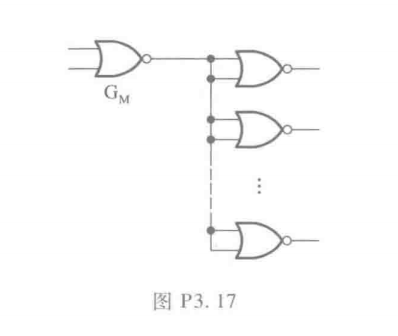
\includegraphics[width=0.4\textwidth]{3.17.png}
\end{center}
\textbf{题3.17电路图}

\subsubsection{解答}
扇出数由低电平驱动能力和高电平驱动能力的最小值决定：
\begin{enumerate}
    \item \textbf{低电平扇出数$N_L$}：

每个负载或非门有2个输入端，低电平输入电流为$|I_{IL}|=1.6mA$，总电流为$N \times 2 \times 1.6mA$，需满足：
\[
N_L \times 2 \times 1.6mA \le I_{OL(max)} = 16mA \implies N_L \le 5
\]

    \item \textbf{高电平扇出数$N_H$}：

每个负载或非门有2个输入端，高电平输入电流为$I_{IH}=40\mu A$，总电流为$N \times 2 \times 40\mu A$，需满足：
\[
N_H \times 2 \times 40\mu A \le |I_{OH(max)}| = 0.4mA \implies N_H \le 5
\]
\end{enumerate}

最终扇出数取最小值：
\[
N = \min(N_L, N_H) = 5
\]

\subsection{题3.23：OC门驱动三极管电路分析}
\subsubsection{题目}
在下图(a)所示电路中已知三极管导通时$V_{BE}=0.7V$，饱和压降$V_{CE(sat)}=0.3V$，饱和导通内阻为$R_{CE(sat)}=20\Omega$，三极管的电流放大系数$\beta=100$。OC门$G_1$输出截止时的漏电流约为50$\mu$A，导通时允许的最大负载电流为16mA，输出低电平$\le 0.3V$。$G_2 \sim G_5$均为74系列TTL电路，其中$G_2$为反相器，$G_3$和$G_4$是与非门，$G_5$是或非门，它们的输入特性如图(b)所示。试问：
\begin{enumerate}
    \item 在三极管集电极输出的高、低电压满足$V_{OH} \ge 3.5V, V_{OL} \le 0.3V$的条件下，$R_B$的取值范围有多大？
    \item 若将OC门改成推挽式输出的TTL门电路，会发生什么问题？
\end{enumerate}

\begin{center}
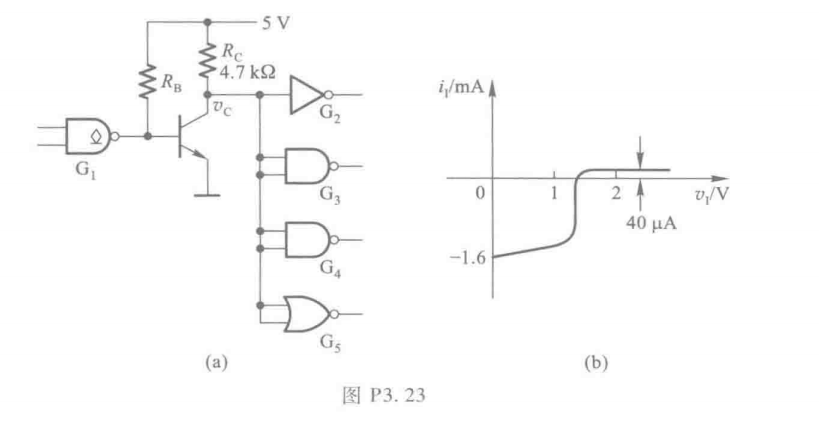
\includegraphics[width=0.7\textwidth]{3.23.png}
\end{center}
\textbf{题3.23电路图与输入特性}

\subsubsection{解答}
\paragraph{(1) $R_B$取值范围计算}
\begin{itemize}
    \item \textbf{三极管饱和导通条件}：基极电流$I_B \ge I_{BS} = \dfrac{I_{CS}}{\beta}$

$I_{CS} = \dfrac{V_{CC} - V_{CE(sat)}}{R_C} + 4|I_{IL}|$（4个负载门的低电平输入电流）

代入数据：
$I_{CS} = \dfrac{5-0.3}{4.7k\Omega} + 4 \times 1.6mA \approx 1mA + 6.4mA = 7.4mA$

$I_{BS} = 7.4mA / 100 = 74\mu A$

基极电流由OC门导通时提供：
$I_B = \dfrac{V_{CC} - V_{BE} - V_{OL}}{R_B} \ge I_{BS}$

解得：
$R_B \le \dfrac{5-0.7-0.3}{74\mu A} \approx 54k\Omega$

    \item \textbf{三极管截止条件}：OC门截止时，漏电流$I_{OH}=50\mu A$，基极电位$V_B \le 0$，即：
$I_{OH} \times R_B \le V_{BE} \implies R_B \le \dfrac{0.7V}{50\mu A} = 14k\Omega$

同时OC门导通时负载电流不超过最大值：
$\dfrac{5-0.7-0.3}{R_B} \le 16mA \implies R_B \ge \dfrac{4V}{16mA} = 250\Omega$
\end{itemize}

综合得：
\[
250\Omega \le R_B \le 14k\Omega
\]

\paragraph{(2) 推挽式TTL门的问题}
推挽式输出的TTL门无法承受OC门的线与特性，当输出为低电平时，三极管基极电流会灌入TTL门的输出级，导致输出管过流损坏；且推挽输出无法实现线与逻辑，不能直接驱动三极管基极。
\newpage

\section{第四章 组合逻辑电路 作业}
% 这是子文件，可直接用 \input{文件名} 引入主文档

\subsection{题4.3：组合逻辑电路功能分析}
\subsubsection{题目}
分析图 P4.3 电路的逻辑功能，写出 $Y_1$、$Y_2$ 的逻辑函数式，列出真值表，指出电路完成什么逻辑功能。

\begin{center}
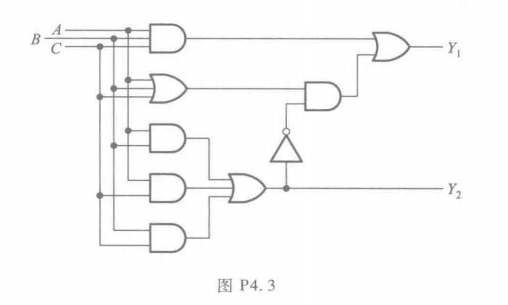
\includegraphics[width=0.6\textwidth]{4.3.png}
\end{center}
题4.3 逻辑电路图

\subsubsection{解答}
\begin{enumerate}
    \item \textbf{写出逻辑表达式}
    \begin{itemize}
        \item 由电路图逐级推导输出逻辑函数：
        \[
        Y_2 = AB + BC + AC
        \]
        \[
        Y_1 = ABC + (A+B+C) \cdot \overline{Y_2}
        \]
        \item 代入 $Y_2$ 并化简：
        \[
        \begin{aligned}
        Y_1 &= ABC + (A+B+C)\overline{AB+BC+AC} \\
        &= A\overline{B}\overline{C} + \overline{A}B\overline{C} + \overline{A}\overline{B}C + ABC \\
        &= A \oplus B \oplus C
        \end{aligned}
        \]
        \item 最终最简逻辑式：
        \[
        \boxed{Y_1 = A \oplus B \oplus C,\quad Y_2 = AB + BC + AC}
        \]
    \end{itemize}

    \item \textbf{列出真值表}
    \begin{center}
    \begin{tabular}{ccc|cc}
        \toprule
        $A$ & $B$ & $C$ & $Y_1$ & $Y_2$ \\
        \midrule
        0 & 0 & 0 & 0 & 0 \\
        0 & 0 & 1 & 1 & 0 \\
        0 & 1 & 0 & 1 & 0 \\
        0 & 1 & 1 & 0 & 1 \\
        1 & 0 & 0 & 1 & 0 \\
        1 & 0 & 1 & 0 & 1 \\
        1 & 1 & 0 & 0 & 1 \\
        1 & 1 & 1 & 1 & 1 \\
        \bottomrule
    \end{tabular}
    \end{center}

    \item \textbf{逻辑功能分析}
    \begin{itemize}
        \item $Y_1 = A \oplus B \oplus C$：三变量异或，为 \textbf{全加器和位}，输入 1 的个数为奇数时输出为 1。
        \item $Y_2 = AB+BC+AC$：多数表决逻辑，为 \textbf{全加器进位位}，输入 1 的个数大于等于 2 时输出为 1。
        \item 整个电路为标准 \textbf{1 位全加器}，$Y_1$ 为和位 $S$，$Y_2$ 为进位输出 $C_O$。
    \end{itemize}
\end{enumerate}

\subsection{题4.5：用与非门设计四变量多数表决电路}
\subsubsection{题目}
用与非门设计四变量的多数表决电路。当输入变量 $A$、$B$、$C$、$D$ 有 3 个或 3 个以上为 1 时输出为 1，输入为其他状态时输出为 0。

\subsubsection{解答}
\begin{enumerate}
    \item \textbf{列出真值表}
    \begin{center}
    \begin{tabular}{cccc|c}
        \toprule
        $A$ & $B$ & $C$ & $D$ & $Y$ \\
        \midrule
        0 & 0 & 0 & 0 & 0 \\
        0 & 0 & 0 & 1 & 0 \\
        0 & 0 & 1 & 0 & 0 \\
        0 & 0 & 1 & 1 & 0 \\
        0 & 1 & 0 & 0 & 0 \\
        0 & 1 & 0 & 1 & 0 \\
        0 & 1 & 1 & 0 & 0 \\
        0 & 1 & 1 & 1 & 1 \\
        1 & 0 & 0 & 0 & 0 \\
        1 & 0 & 0 & 1 & 0 \\
        1 & 0 & 1 & 0 & 0 \\
        1 & 0 & 1 & 1 & 1 \\
        1 & 1 & 0 & 0 & 0 \\
        1 & 1 & 0 & 1 & 1 \\
        1 & 1 & 1 & 0 & 1 \\
        1 & 1 & 1 & 1 & 1 \\
        \bottomrule
    \end{tabular}
    \end{center}

    \item \textbf{写出逻辑表达式并化简为与非-与非形式}
    \begin{itemize}
        \item 从真值表写出标准最小项和式：
        \[
        Y = \sum m(7,11,13,14,15)
        \]
        \item 卡诺图化简得到最简与或式：
        \[
        Y = ABC + ABD + ACD + BCD
        \]
        \item 两次取反转换为与非-与非形式：
        \[
        Y = \overline{\overline{ABC + ABD + ACD + BCD}}
        = \overline{\overline{ABC} \cdot \overline{ABD} \cdot \overline{ACD} \cdot \overline{BCD}}
        \]
    \end{itemize}

    \item \textbf{逻辑功能分析}
    \begin{itemize}
        \item 输入 $A,B,C,D$ 中有 3 个或 4 个为 1 时输出 1，否则输出 0，实现 \textbf{四变量多数表决器}。
        \item 表达式已化为与非-与非形式，可直接用两级与非门实现。
    \end{itemize}
\end{enumerate}

\subsection{题4.6：水箱水泵控制逻辑电路设计}
\subsubsection{题目}
有一水箱由大、小两台水泵 $M_L$ 和 $M_S$ 供水，如图 P4.6 所示。水箱中设置了 3 个水位检测元件 A、B、C。水面低于检测元件时，检测元件给出高电平；水面高于检测元件时，检测元件给出低电平。现要求：
\begin{itemize}
    \item 当水位超过 C 点时水泵停止工作；
    \item 水位低于 C 点而高于 B 点时 $M_S$ 单独工作；
    \item 水位低于 B 点而高于 A 点时 $M_L$ 单独工作；
    \item 水位低于 A 点时 $M_L$ 和 $M_S$ 同时工作。
\end{itemize}
试用门电路设计一个控制两台水泵的逻辑电路，要求电路尽量简单。

\begin{center}
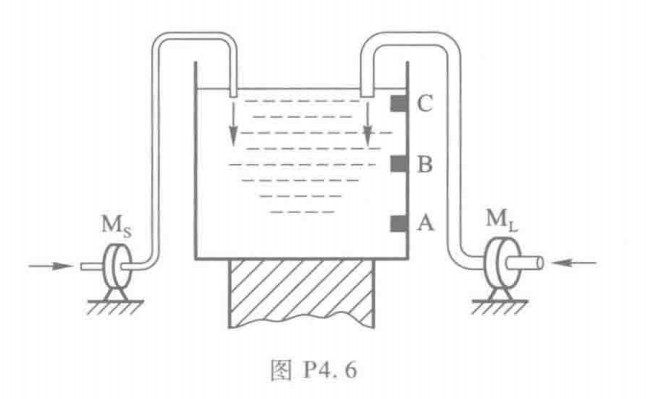
\includegraphics[width=0.6\textwidth]{4.6.png}
\end{center}
题4.6 水箱水泵控制示意图

\subsubsection{解答}
\begin{enumerate}
    \item \textbf{定义逻辑变量}
    \begin{itemize}
        \item 输入：$A,B,C$，高电平（1）表示水位低于该点，低电平（0）表示高于该点。
        \item 输出：$M_L$（大泵）、$M_S$（小泵），1=工作，0=停止。
    \end{itemize}

    \item \textbf{列出真值表（含所有输入状态与无关项）}
    \begin{center}
    \begin{tabular}{ccc|cc|c}
        \toprule
        $A$ & $B$ & $C$ & $M_L$ & $M_S$ & 工作状态 \\
        \midrule
        0 & 0 & 0 & 0 & 0 & 超过C点，全停 \\
        0 & 0 & 1 & 0 & 1 & B~C之间，仅$M_S$工作 \\
        0 & 1 & 0 & \multicolumn{2}{c}{×} & 不可能状态（无关项） \\
        0 & 1 & 1 & 1 & 0 & A~B之间，仅$M_L$工作 \\
        1 & 0 & 0 & \multicolumn{2}{c}{×} & 不可能状态（无关项） \\
        1 & 0 & 1 & \multicolumn{2}{c}{×} & 不可能状态（无关项） \\
        1 & 1 & 0 & \multicolumn{2}{c}{×} & 不可能状态（无关项） \\
        1 & 1 & 1 & 1 & 1 & 低于A点，双泵工作 \\
        \bottomrule
    \end{tabular}
    \end{center}

    \item \textbf{写出逻辑表达式并化简}
    \begin{itemize}
        \item 对 $M_L$ 化简：
        \[
        M_L = B
        \]
        \item 对 $M_S$ 化简：
        \[
        M_S = \overline{B}C
        \]
        \item 验证：
        \begin{itemize}
            \item 水位超过C：$A=B=C=0 \Rightarrow M_L=0,\ M_S=0$（正确）
            \item 水位B~C间：$A=0,B=0,C=1 \Rightarrow M_L=0,\ M_S=1$（正确）
            \item 水位A~B间：$A=0,B=1,C=1 \Rightarrow M_L=1,\ M_S=0$（正确）
            \item 水位低于A：$A=1,B=1,C=1 \Rightarrow M_L=1,\ M_S=1$（正确）
        \end{itemize}
    \end{itemize}

    \item \textbf{逻辑电路图说明}
    \begin{itemize}
        \item $M_L = B$：直接由输入 $B$ 控制，无需门电路。
        \item $M_S = \overline{B}C$：使用一个**非门**（对B取反）和一个**与门**（连接$\overline{B}$和C）实现。
        \item 整体电路最简，完全满足题目所有控制要求。
    \end{itemize}
\end{enumerate}

\subsection{题4.12：用74HC138实现多输出逻辑函数}
\subsubsection{题目}
试画出用3线-8线译码器74HC138（见图4.4.7）和门电路产生如下多输出逻辑函数的逻辑图。
\[
\begin{cases}
Y_1 = AC \\
Y_2 = \overline{A}\overline{B}C + A\overline{B}\overline{C} + BC \\
Y_3 = \overline{B}\overline{C} + AB\overline{C}
\end{cases}
\]

\begin{center}
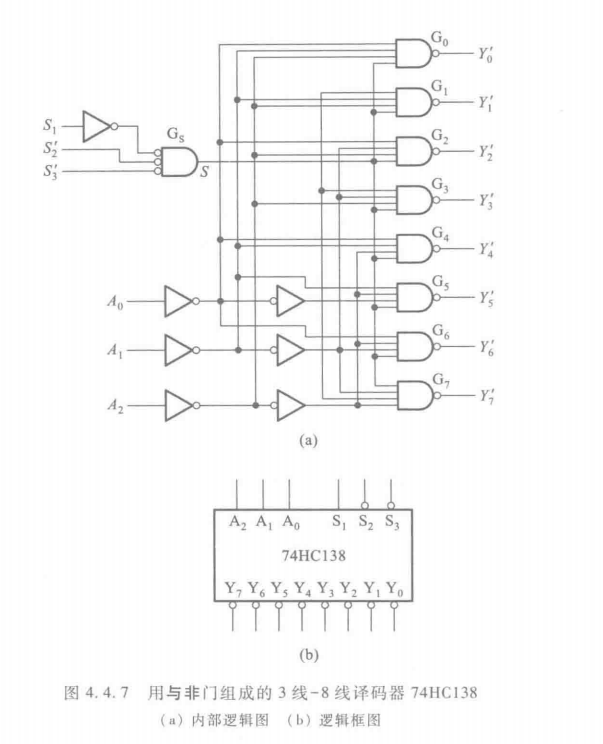
\includegraphics[width=0.6\textwidth]{4.4.7.png}
\end{center}
图4.4.7 74HC138逻辑符号

\subsubsection{解答}
\begin{enumerate}
    \item \textbf{将函数转换为标准与或式（最小项和形式）}
    \begin{itemize}
        \item 令地址高位到低位：$A_2=A,\ A_1=B,\ A_0=C$。
        \item $Y_1 = AC = A(B+\overline{B})C = ABC + A\overline{B}C = \sum m(5,7)$
        \item $Y_2 = \overline{A}\overline{B}C + A\overline{B}\overline{C} + BC
        = \overline{A}\overline{B}C + A\overline{B}\overline{C} + \overline{A}BC + ABC
        = \sum m(1,3,4,7)$
        \item $Y_3 = \overline{B}\overline{C} + AB\overline{C}
        = \overline{A}\overline{B}\overline{C} + A\overline{B}\overline{C} + AB\overline{C}
        = \sum m(0,4,6)$
    \end{itemize}

    \item \textbf{利用译码器输出实现逻辑函数}
    \begin{itemize}
        \item 74HC138 输出低电平有效：$\overline{Y_i} = \overline{m_i}$。
        \item 或运算转为与非形式：$\displaystyle Y=\sum m_i = \overline{\prod \overline{m_i}}$。
        \[
        Y_1 = \sum m(5,7) = \overline{\overline{Y_5} \cdot \overline{Y_7}}
        \]
        \[
        Y_2 = \sum m(1,3,4,7) = \overline{\overline{Y_1} \cdot \overline{Y_3} \cdot \overline{Y_4} \cdot \overline{Y_7}}
        \]
        \[
        Y_3 = \sum m(0,4,6) = \overline{\overline{Y_0} \cdot \overline{Y_4} \cdot \overline{Y_6}}
        \]
    \end{itemize}

    \item \textbf{逻辑电路连接说明}
    \begin{itemize}
        \item 输入 $A,B,C$ 分别接 74HC138 地址端 $A_2,A_1,A_0$；
        \item 使能端 $S_1$ 接高电平，$\overline{S_2},\overline{S_3}$ 接低电平，译码器正常工作；
        \item 外接与非门对对应译码器输出做与非运算，即可实现 $Y_1,Y_2,Y_3$。
    \end{itemize}
\end{enumerate}

\subsection{题4.16：用74HC151数据选择器实现逻辑函数}
\subsubsection{题目}
分析图 P4.16 电路，写出输出 $Z$ 的逻辑函数式。74HC151 为 8 选 1 数据选择器，它的逻辑图见图 4.5.5，输出的逻辑函数式见式(4.5.6)。

\begin{center}
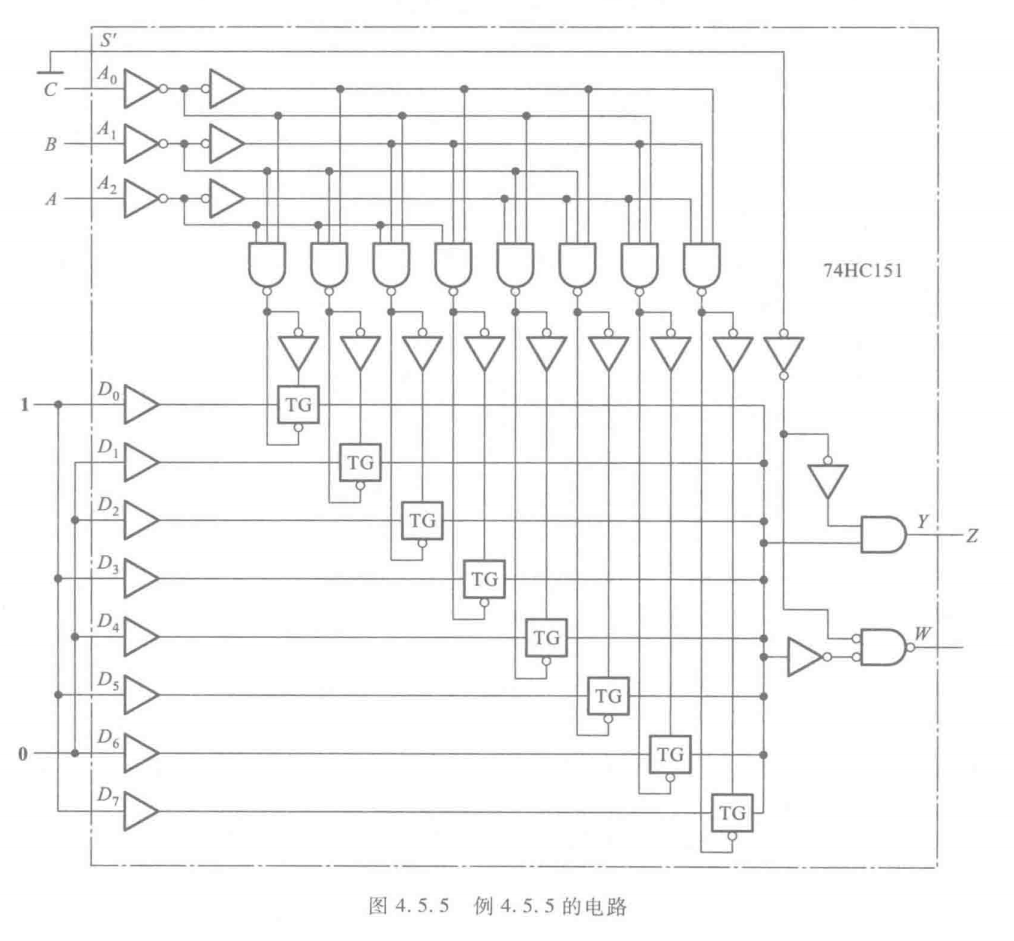
\includegraphics[width=0.6\textwidth]{4.5.5.png}
\end{center}
图4.5.5 74HC151逻辑符号

\begin{center}
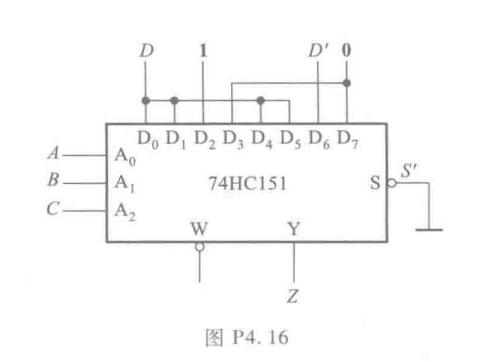
\includegraphics[width=0.6\textwidth]{4.16.png}
\end{center}
图P4.16 电路示意图

\subsubsection{解答}
\begin{enumerate}
    \item \textbf{分析数据选择器输入与输出关系}
    \begin{itemize}
        \item 74HC151 输出表达式：
        \[
        Y = \sum_{i=0}^{7} m_i D_i
        \]
        $m_i$ 为地址 $A_2A_1A_0$ 最小项，$D_i$ 为数据输入。
        \item 地址：$A_2=C,\ A_1=B,\ A_0=A$。
        \item 数据输入：
        \[
        D_0=D,\ D_1=D,\ D_2=1,\ D_3=1,\ D_4=\overline{D},\ D_5=\overline{D},\ D_6=0,\ D_7=0
        \]
        \item 使能端低电平有效，芯片工作，$Z=Y$。
    \end{itemize}

    \item \textbf{写出并化简输出逻辑函数}
    \begin{itemize}
        \item 代入展开：
        \[
        \begin{aligned}
        Z &= \overline{C}\overline{B}\overline{A}D + \overline{C}\overline{B}A D
        + \overline{C}B\overline{A} \cdot 1 + \overline{C}B A \cdot 1 \\
        &\quad + C\overline{B}\overline{A}\overline{D} + C\overline{B}A \overline{D}
        \end{aligned}
        \]
        \item 合并化简：
        \[
        Z = \overline{C}\overline{B}D + \overline{C}B + C\overline{B}\overline{D}
        \]
    \end{itemize}

    \item \textbf{逻辑功能分析}
    \begin{itemize}
        \item 电路实现四变量逻辑函数 $Z(A,B,C,D) = \overline{C}\overline{B}D + \overline{C}B + C\overline{B}\overline{D}$，由 8 选 1 数据选择器直接实现。
    \end{itemize}
\end{enumerate}

\subsection{题4.18：用4选1数据选择器产生逻辑函数}
\subsubsection{题目}
试用4选1数据选择器产生逻辑函数：
\[
Y = A\overline{B}\overline{C} + \overline{A}\overline{C} + BC
\]

\subsubsection{解答}
\begin{enumerate}
    \item \textbf{将函数转换为标准与或式}
    \begin{itemize}
        \item 展开为最小项：
        \[
        \begin{aligned}
        Y &= A\overline{B}\overline{C} + \overline{A}(B+\overline{B})\overline{C} + (A+\overline{A})BC \\
        &= A\overline{B}\overline{C} + \overline{A}B\overline{C} + \overline{A}\overline{B}\overline{C}
        + ABC + \overline{A}BC \\
        &= \sum m(0,1,2,3,6,7)
        \end{aligned}
        \]
    \end{itemize}

    \item \textbf{选择地址变量并确定数据输入}
    \begin{itemize}
        \item 取地址 $A_1=A,\ A_0=B$，4选1输出：
        \[
        Y = \overline{A}\overline{B}D_0 + \overline{A}B D_1 + A\overline{B}D_2 + AB D_3
        \]
        \item 按变量分组：
        \[
        Y = \overline{A}\overline{B}\,\overline{C} + \overline{A}B \cdot 1 + A\overline{B}\,\overline{C} + AB \cdot 1
        \]
        \item 对应数据输入：
        \[
        D_0 = \overline{C},\quad D_1 = 1,\quad D_2 = \overline{C},\quad D_3 = 1
        \]
    \end{itemize}

    \item \textbf{电路实现说明}
    \begin{itemize}
        \item 地址 $A,B$ 接选择器地址端 $A_1,A_0$；
        \item $D_0,D_2$ 接 $\overline{C}$，$D_1,D_3$ 接高电平；
        \item 使能端接地，即可实现给定逻辑函数。
    \end{itemize}
\end{enumerate}

\subsection{题4.23：用74HC151实现双功能控制电路}
\subsubsection{题目}
用8选1数据选择器74HC151设计一个组合逻辑电路。该电路有3个输入逻辑变量 $A,B,C$ 和1个工作状态控制变量 $M$。
当 $M=0$ 时实现“意见一致”功能（$A,B,C$ 状态一致时输出为1）；
当 $M=1$ 时实现“多数表决”功能。

\begin{center}
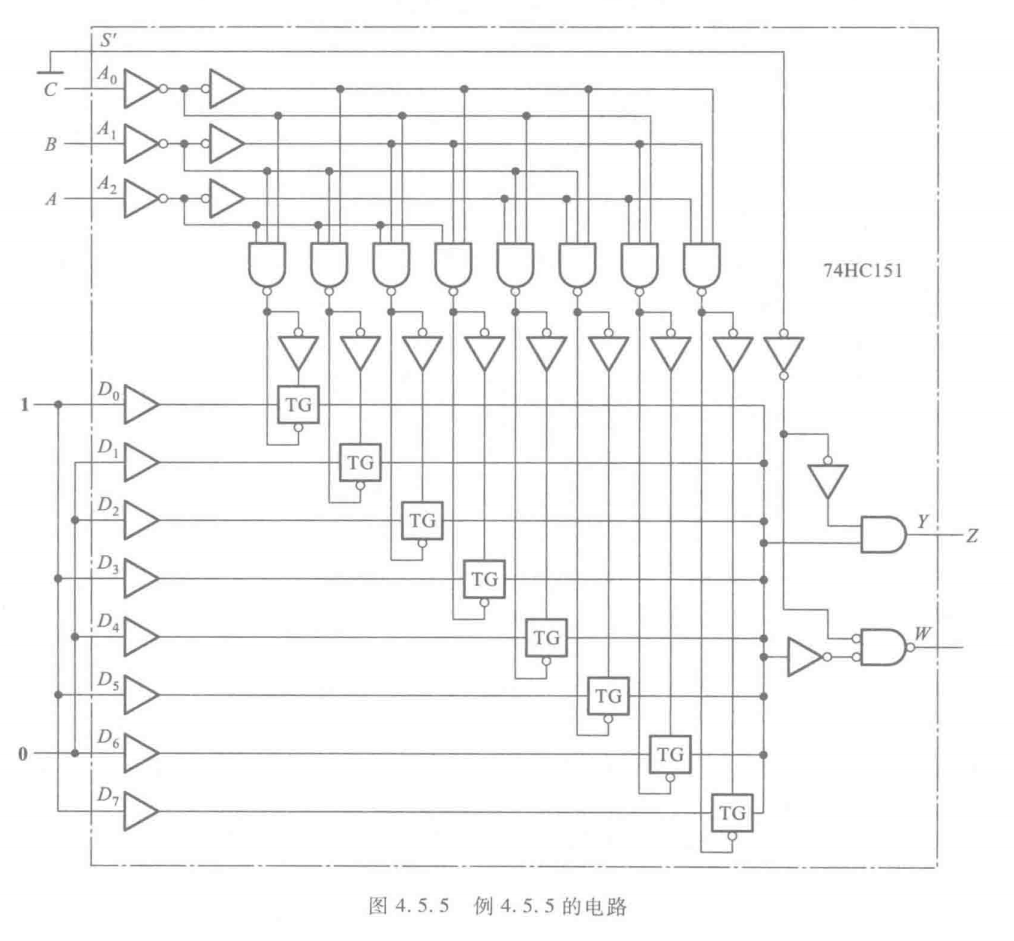
\includegraphics[width=0.6\textwidth]{4.5.5.png}
\end{center}
图4.5.5 74HC151逻辑符号

\subsubsection{解答}
\begin{enumerate}
    \item \textbf{列出输出逻辑函数的真值表}
    \begin{center}
    \begin{tabular}{cccc|c}
        \toprule
        $M$ & $A$ & $B$ & $C$ & $Y$ \\
        \midrule
        0 & 0 & 0 & 0 & 1 \\
        0 & 0 & 0 & 1 & 0 \\
        0 & 0 & 1 & 0 & 0 \\
        0 & 0 & 1 & 1 & 0 \\
        0 & 1 & 0 & 0 & 0 \\
        0 & 1 & 0 & 1 & 0 \\
        0 & 1 & 1 & 0 & 0 \\
        0 & 1 & 1 & 1 & 1 \\
        1 & 0 & 0 & 0 & 0 \\
        1 & 0 & 0 & 1 & 0 \\
        1 & 0 & 1 & 0 & 0 \\
        1 & 0 & 1 & 1 & 1 \\
        1 & 1 & 0 & 0 & 0 \\
        1 & 1 & 0 & 1 & 1 \\
        1 & 1 & 1 & 0 & 1 \\
        1 & 1 & 1 & 1 & 1 \\
        \bottomrule
    \end{tabular}
    \end{center}

    \item \textbf{选择地址变量并确定数据输入}
    \begin{itemize}
        \item 地址端 $A_2=A,\ A_1=B,\ A_0=C$；
        \[
        Y = \sum_{i=0}^{7} m_i D_i
        \]
        \item 由真值表得：
        \[
        \begin{aligned}
        D_0 &= 1,\quad D_1 = 0,\quad D_2 = 0,\quad D_3 = M \\
        D_4 &= 0,\quad D_5 = M,\quad D_6 = M,\quad D_7 = 1
        \end{aligned}
        \]
    \end{itemize}

    \item \textbf{电路实现说明}
    \begin{itemize}
        \item $A,B,C$ 接 74HC151 地址输入端 $A_2,A_1,A_0$；
        \item 数据端按 $D_0\sim D_7$ 分别接 $1,0,0,M,0,M,M,1$；
        \item 使能端接地，芯片工作，由 $M$ 切换两种逻辑功能。
    \end{itemize}
\end{enumerate}

% 仅子章节内容，宏包统一在主文件导入
\section{触发器基础题}

% 题 5.1
\subsection{题 5.1：与非门 SR 锁存器波形}

题目：画出图中由与非门组成的 SR 锁存器输出端 $Q$、$\overline{Q}$ 的电压波形，输入端 $\overline{S_D}$、$\overline{R_D}$ 的电压波形如图中所示。

\begin{center}
    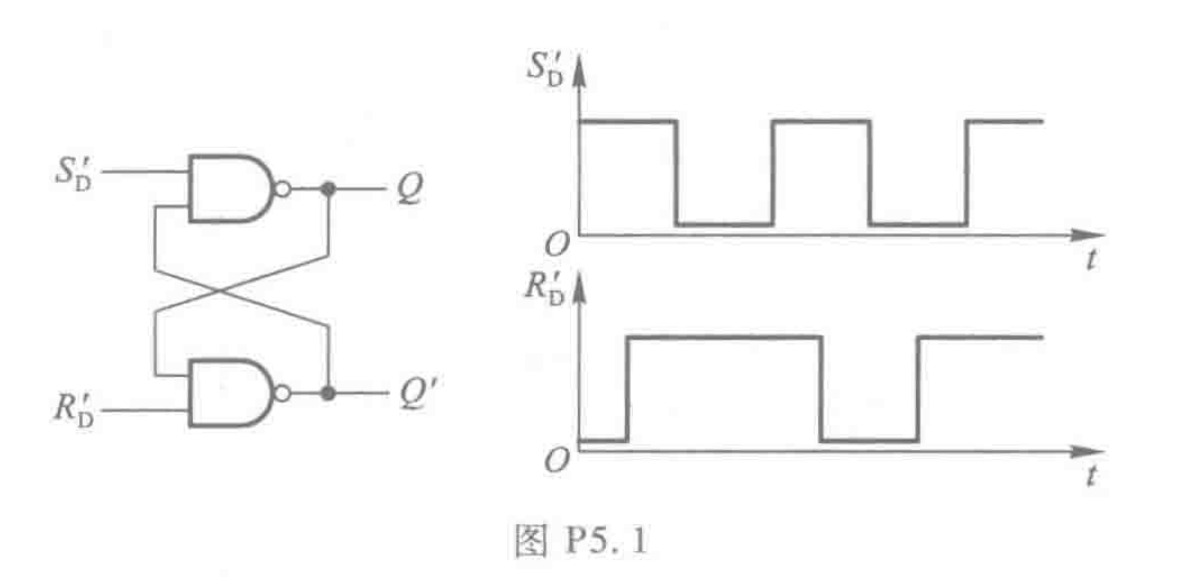
\includegraphics[width=0.45\textwidth]{5.1.png}
\end{center}

\textbf{解答：}

与非门构成的 SR 锁存器为低电平有效，特性表如下：

\begin{center}
\begin{tabular}{cccc}
\toprule
$\overline{S_D}$ & $\overline{R_D}$ & $Q$ & 功能 \\
\midrule
1 & 1 & 保持 & 锁存 \\
1 & 0 & 0 & 置 0（复位）\\
0 & 1 & 1 & 置 1（置位）\\
0 & 0 & 不定 & 禁止态 \\
\bottomrule
\end{tabular}
\end{center}

设初始状态 $Q=0$，根据输入波形逐段分析：
\begin{enumerate}
    \item $\overline{S_D}=1,\ \overline{R_D}=0$：置 0，$Q=0$
    \item $\overline{S_D}=1,\ \overline{R_D}=1$：保持，$Q=0$
    \item $\overline{S_D}=0,\ \overline{R_D}=1$：置 1，$Q=1$
    \item $\overline{S_D}=1,\ \overline{R_D}=1$：保持，$Q=1$
    \item $\overline{S_D}=0,\ \overline{R_D}=0$：禁止态，$Q$ 与 $\overline{Q}$ 均为 1
    \item $\overline{S_D}=1,\ \overline{R_D}=1$：恢复保持，状态取决于优先解除禁止的输入端
\end{enumerate}

% 手绘标准时序波形图
\begin{center}
\begin{tikzpicture}[scale=0.7,line width=0.7pt]
% 纵坐标标注
\foreach \y/\lab in {6/$\overline{S_D}$,4/$\overline{R_D}$,2/$Q$,0/$\overline{Q}$}
    \node[left] at (-0.5,\y) {\lab};
% 时间刻度
\foreach \x in {0,1,2,3,4,5,6,7,8}
    \draw (\x,7) -- (\x,-1);

% 绘制SD非波形
\draw (0,6) -- (2,6) -- (2,5) -- (3,5) -- (3,6) -- (5,6) -- (5,5) -- (6,5) -- (6,6) -- (8,6);
% 绘制RD非波形
\draw (0,5) -- (1,5) -- (1,4) -- (4,4) -- (4,5) -- (6,5) -- (6,4) -- (8,4);
% 绘制Q波形
\draw (0,2) -- (3,2) -- (3,3) -- (5,3) -- (6,3) -- (6,2.5) -- (8,2);
% 绘制Q非波形
\draw (0,3) -- (3,3) -- (3,2) -- (5,2) -- (6,2) -- (6,2.5) -- (8,3);

% 高低电平标注
\node[right] at (8.2,6) {高};
\node[right] at (8.2,5) {低};
\end{tikzpicture}
\end{center}

\textbf{结论：}
\begin{itemize}
    \item $\overline{S_D}$ 低电平置 1，$\overline{R_D}$ 低电平置 0，均为高电平时保持。
    \item 除禁止态外，$\overline{Q}$ 与 $Q$ 始终互补。
\end{itemize}

\vspace{1em}
\hrulefill
\vspace{1em}

% 题 5.2
\subsection{题 5.2：或非门 SR 锁存器波形}

题目：画出图中由或非门组成的 SR 锁存器输出端 $Q$、$\overline{Q}$ 的电压波形，输入端 $S_D$、$R_D$ 的电压波形如图中所示。

\begin{center}
    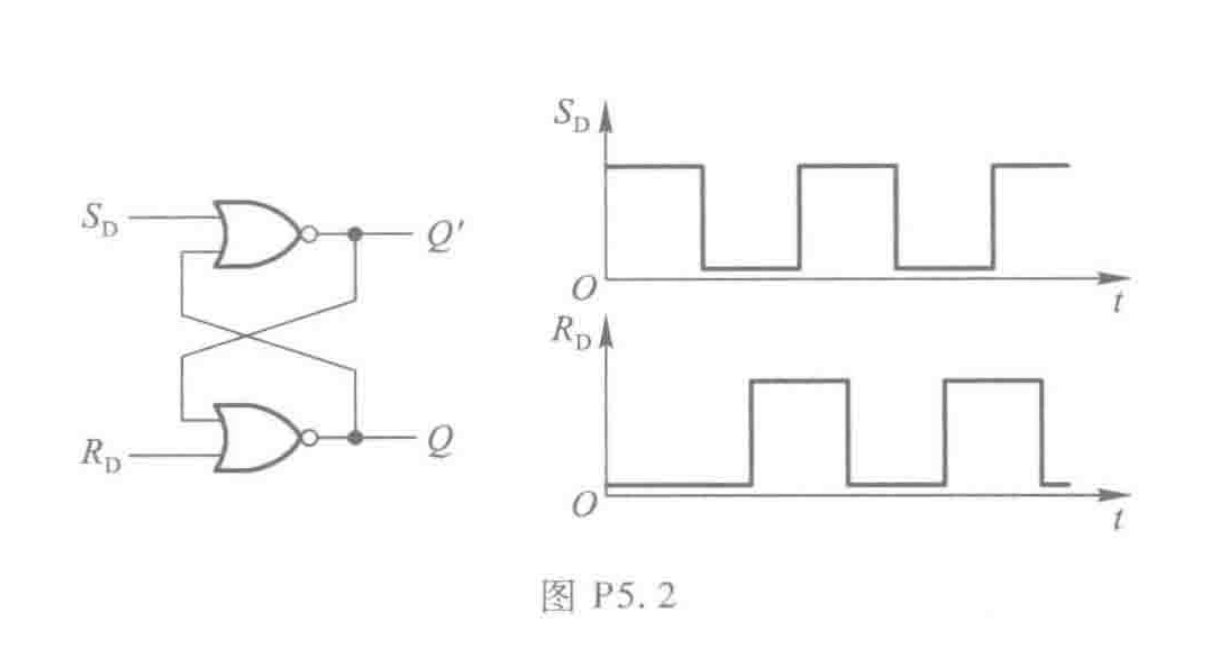
\includegraphics[width=0.45\textwidth]{5.2.png}
\end{center}

\textbf{解答：}

或非门构成的 SR 锁存器为高电平有效，特性表如下：

\begin{center}
\begin{tabular}{cccc}
\toprule
$S_D$ & $R_D$ & $Q$ & 功能 \\
\midrule
0 & 0 & 保持 & 锁存 \\
0 & 1 & 0 & 置 0（复位）\\
1 & 0 & 1 & 置 1（置位）\\
1 & 1 & 不定 & 禁止态 \\
\bottomrule
\end{tabular}
\end{center}

设初始状态 $Q=0$，逐段分析：
\begin{enumerate}
    \item $S_D=1,\ R_D=0$：置 1，$Q=1$
    \item $S_D=0,\ R_D=0$：保持，$Q=1$
    \item $S_D=0,\ R_D=1$：置 0，$Q=0$
    \item $S_D=1,\ R_D=0$：置 1，$Q=1$
    \item $S_D=0,\ R_D=1$：置 0，$Q=0$
\end{enumerate}

% 时序波形图
\begin{center}
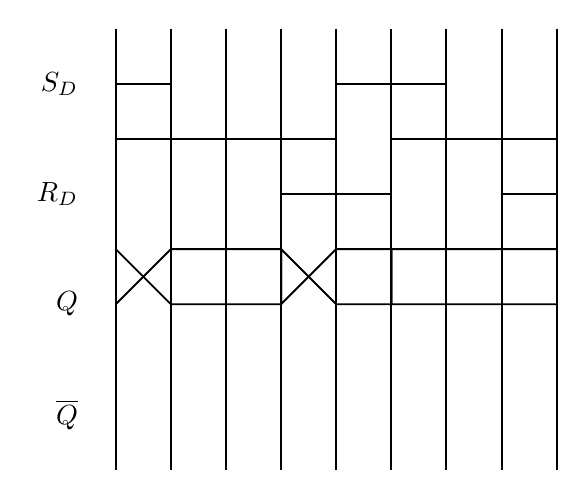
\begin{tikzpicture}[scale=0.7,line width=0.7pt]
\foreach \y/\lab in {6/$S_D$,4/$R_D$,2/$Q$,0/$\overline{Q}$}
    \node[left] at (-0.5,\y) {\lab};
\foreach \x in {0,1,2,3,4,5,6,7,8}
    \draw (\x,7) -- (\x,-1);

\draw (0,6) -- (1,6) -- (1,5) -- (4,5) -- (4,6) -- (6,6) -- (6,5) -- (8,5);
\draw (0,5) -- (3,5) -- (3,4) -- (5,4) -- (5,5) -- (7,5) -- (7,4) -- (8,4);
\draw (0,2) -- (1,3) -- (3,3) -- (3,2) -- (4,3) -- (5,3) -- (5,2) -- (8,2);
\draw (0,3) -- (1,2) -- (3,2) -- (3,3) -- (4,2) -- (5,2) -- (5,3) -- (8,3);
\end{tikzpicture}
\end{center}

\textbf{结论：}
\begin{itemize}
    \item $S_D=1$ 置 1，$R_D=1$ 置 0，均为 0 时保持。
    \item 除禁止态外，$\overline{Q}$ 与 $Q$ 互补。
\end{itemize}

\vspace{1em}
\hrulefill
\vspace{1em}

% 题 5.9
\subsection{题 5.9：边沿触发 JK 触发器波形}

题目：已知边沿触发 JK 触发器各输入端电压波形如图所示，画出输出 $Q$、$\overline{Q}$ 的波形。

\begin{center}
    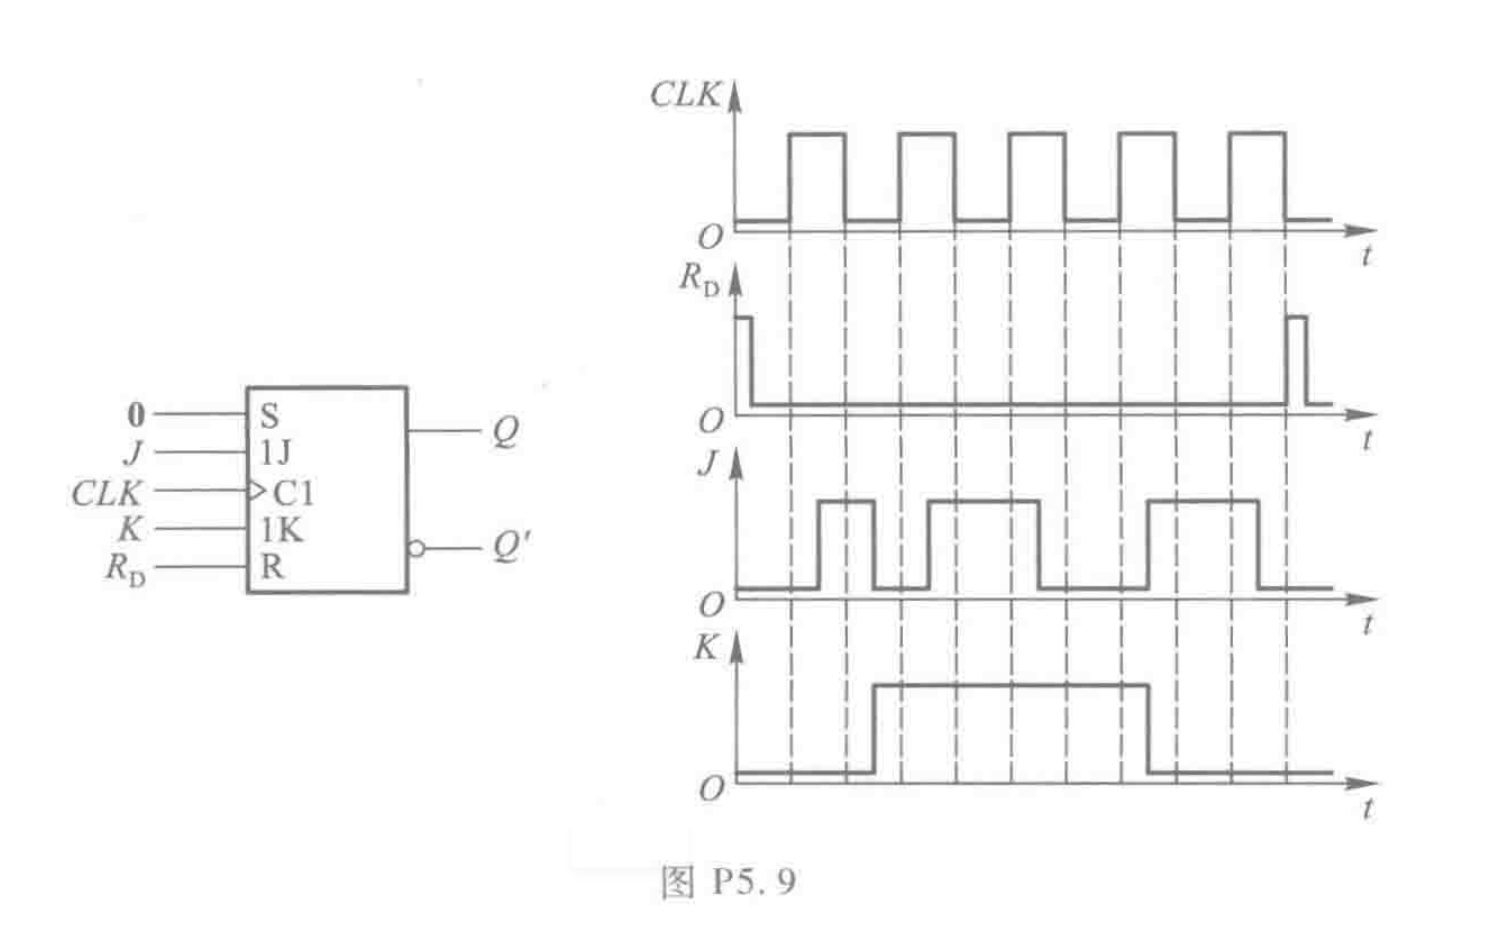
\includegraphics[width=0.5\textwidth]{5.9.png}
\end{center}

\textbf{解答：}

该触发器为 \textbf{下降沿触发} 的 JK 触发器，异步复位端 $\overline{R_D}$ 低电平有效，优先级最高。

特性方程：
\[
Q^{n+1} = J\overline{Q^n} + \overline{K}Q^n
\]

设初始状态 $Q=0$，逐周期分析：
\begin{enumerate}
    \item $\overline{R_D}=0$：强制置 0，$Q=0$
    \item 第 1 个时钟下降沿：$J=0,K=0$，保持 $Q=0$
    \item 第 2 个时钟下降沿：$J=1,K=1$，翻转，$Q=1$
    \item 第 3 个时钟下降沿：$J=1,K=1$，翻转，$Q=0$
    \item 第 4 个时钟下降沿：$J=0,K=1$，置 0，$Q=0$
    \item 第 5 个时钟下降沿：$J=1,K=0$，置 1，$Q=1$
    \item 最后 $\overline{R_D}=0$：强制置 0，$Q=0$
\end{enumerate}

% JK触发器完整时序图
\begin{center}
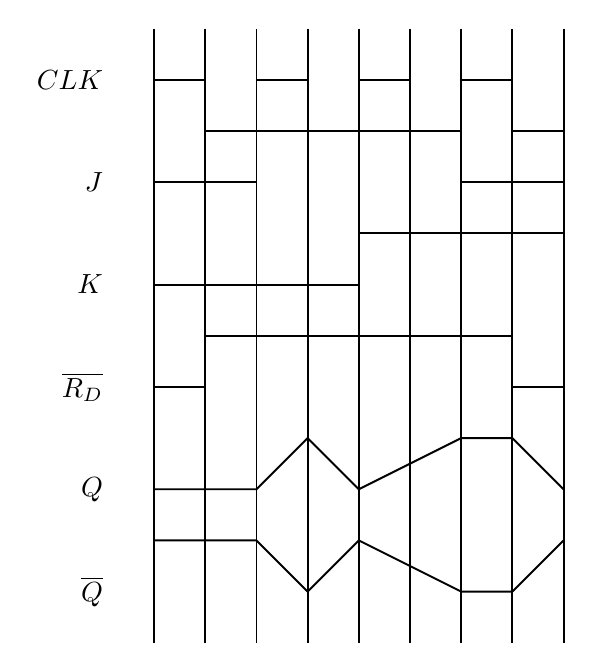
\begin{tikzpicture}[scale=0.65,line width=0.7pt]
\foreach \y/\lab in {8/$CLK$,6/$J$,4/$K$,2/$\overline{R_D}$,0/$Q$,-2/$\overline{Q}$}
    \node[left] at (-0.8,\y) {\lab};
\foreach \x in {0,1,2,3,4,5,6,7,8}
    \draw (\x,9) -- (\x,-3);

% 时钟波形
\draw (0,7)--(0,8)--(1,8)--(1,7)--(2,7)--(2,8)--(3,8)--(3,7)
      --(4,7)--(4,8)--(5,8)--(5,7)--(6,7)--(6,8)--(7,8)--(7,7)--(8,7);
% J波形
\draw (0,6)--(2,6)--(2,7)--(6,7)--(6,6)--(8,6);
% K波形
\draw (0,4)--(4,4)--(4,5)--(8,5);
% 异步复位
\draw (0,2)--(1,2)--(1,3)--(7,3)--(7,2)--(8,2);
% Q输出
\draw (0,0)--(2,0)--(3,1)--(4,0)--(6,1)--(7,1)--(8,0);
% Q非输出
\draw (0,-1)--(2,-1)--(3,-2)--(4,-1)--(6,-2)--(7,-2)--(8,-1);
\end{tikzpicture}
\end{center}

\textbf{结论：}
\begin{itemize}
    \item 状态仅在时钟下降沿更新。
    \item 异步复位 $\overline{R_D}=0$ 可随时强制置 0，与时钟无关。
    \item $\overline{Q}$ 始终与 $Q$ 电平互补。
\end{itemize}

\end{document}